\documentclass[12pt, a4paper, notitlepage]{article}

\usepackage{polski}
\usepackage[utf8]{inputenc}
\usepackage{graphicx}
\usepackage{listings}
\usepackage[usenames]{color}
\usepackage{geometry}
\geometry{inner=15mm, outer=15mm, tmargin=10mm, bmargin=10mm, foot=0mm, head=0mm}
\usepackage{pdfpages}
\usepackage[font=small,labelfont=bf]{caption}

\title{Analiza układu mixer za pomocą języka LOTOS}
\author{Kamil Kos, Marlena Olszewska}
\date{\today}

\definecolor{mygreen}{RGB}{20,150,0} % color values Red, Green, Blue
\definecolor{mylilas}{RGB}{170,55,241}
\lstloadlanguages{TeX}
\lstset{language=Matlab,%
    %basicstyle=\color{red},
    breaklines=true,%
    morekeywords={hide,behaviour,where,exit,noexit},
    keywordstyle=\bfseries,%
    morekeywords=[2]{specification,endspec,process,endproc}, keywordstyle=[2]{\color{mygreen}\bfseries},
    identifierstyle=\color{black},%
    stringstyle=\color{mylilas},
    commentstyle=\color{mygreen},%
    showstringspaces=false,%without this there will be a symbol in the places where there is a space
    %numbers=left,%
    %numberstyle={\tiny \color{black}},% size of the numbers
    %numbersep=9pt, % this defines how far the numbers are from the text
    %emph=[1]{specification,endspec,process,endproc},emphstyle=[1]\color{mygreen}, %some words to emphasise    
}

\begin{document}
{\let\newpage\relax\maketitle}

\thispagestyle{empty}
\begin{figure}[!htb]
	\centering
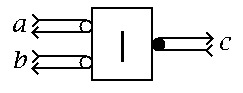
\includegraphics[scale=1]{cd}
\end{figure}

Mixer jest komponentem z trzema dwufazowymi portami: dwoma pasywnymi i jednym aktywnym. \textit{Request} z wejść pasywnych zostaje przeniesiony na port aktywny. Kiedy przychodzi żądanie na port pasywny i mixer nie jest zajęty obsługą innego żądania, przychodzące żądanie zostaje przeniesione na port aktywny (port aktywny staje się \textit{busy}). Gdy port aktywny otrzyma \textit{ack}, port pasywny, z którego żądanie zostało przeniesione także otrzymuje \textit{ack} i~przechodzi w~stan bezczynności (\textit{idle}).
\\\\
Żądanie przychodzące na port pasywny, gdy mixer jest w stanie \textit{busy} (przetwarza żądanie z~drugiego portu pasywnego) nie jest gubione, lecz zostaje obsłużone, gdy mixer będzie bezczynny.
\\\\
Gdy mixer otrzymuje żadania na obu portach jednocześnie, przetworzy najpierw jedno z nich, a drugie później -- wybór żądania jest dowolny. Narzucona jest własność sprawiedliwości -- przy nieskończonej ilości takich sytuacji każdy z portów powinien zostać obsłużony nieskończoną ilość razy.

\newpage
\thispagestyle{empty}
\section*{Specyfikacja w języku LOTOS}
\begin{lstlisting}
specification mixer[ar,br,cr,aa,ba,ca]: noexit
	behaviour
		hide a0,a1,s,b0,b1 in
		(passive[ar,aa,a0,a1]|||passive[br,ba,b0,b1])|[a0,a1,b0,b1]|(trigger[a0,b0,s]|[s]|active[cr,ca,s,a1,b1])
	where
	process active[cr,ca,s,a1,b1]: noexit :=
		(s; cr; ca; a1; active[cr,ca,s,a1,b1])
		[]
		(s; cr; ca; b1; active[cr,ca,s,a1,b1])
	endproc
	
	process trigger[a0,b0,s]: noexit :=
		(a0; s; trigger[a0,b0,s])
		[]
		(b0; s; trigger[a0,b0,s])
	endproc
	
	process passive[req,ack,s0,s1]: noexit :=
		req; s0; s1; ack; passive[req,ack,s0,s1]
	endproc
endspec


\end{lstlisting}

\begin{figure}[!htb]
	\centering
	\begin{minipage}{\linewidth}
	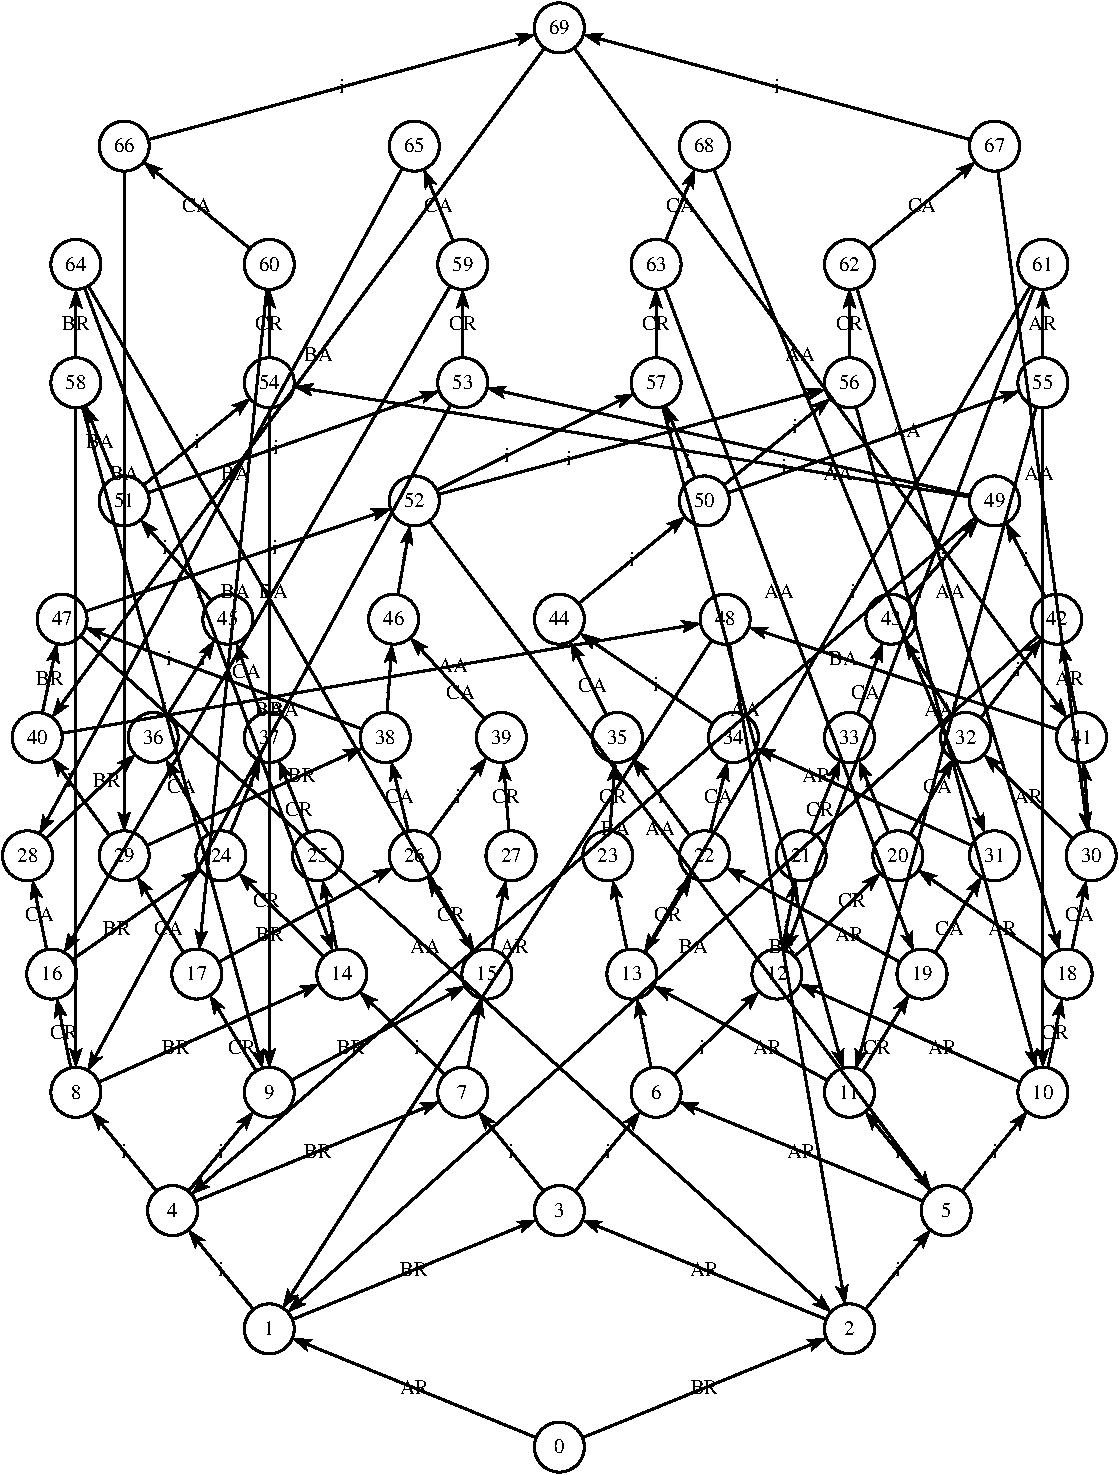
\includegraphics[angle=-90,scale=0.65]{mixer1}
	\captionof{figure}{Etykietowany graf przejść (LTS) dla modelu mixer.lotos}
	\end{minipage}
\end{figure}


\newpage
\thispagestyle{empty}
\begin{figure}[!htb]

	\begin{minipage}{\linewidth}
	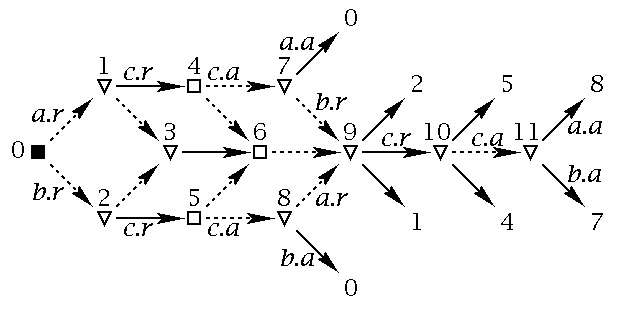
\includegraphics[scale=0.85]{mixer.jpg}
	\captionof{figure}{Specyfikacja za pomocą grafu XDI}
	\end{minipage}

	\vspace{5mm}

	\begin{minipage}{\linewidth}
	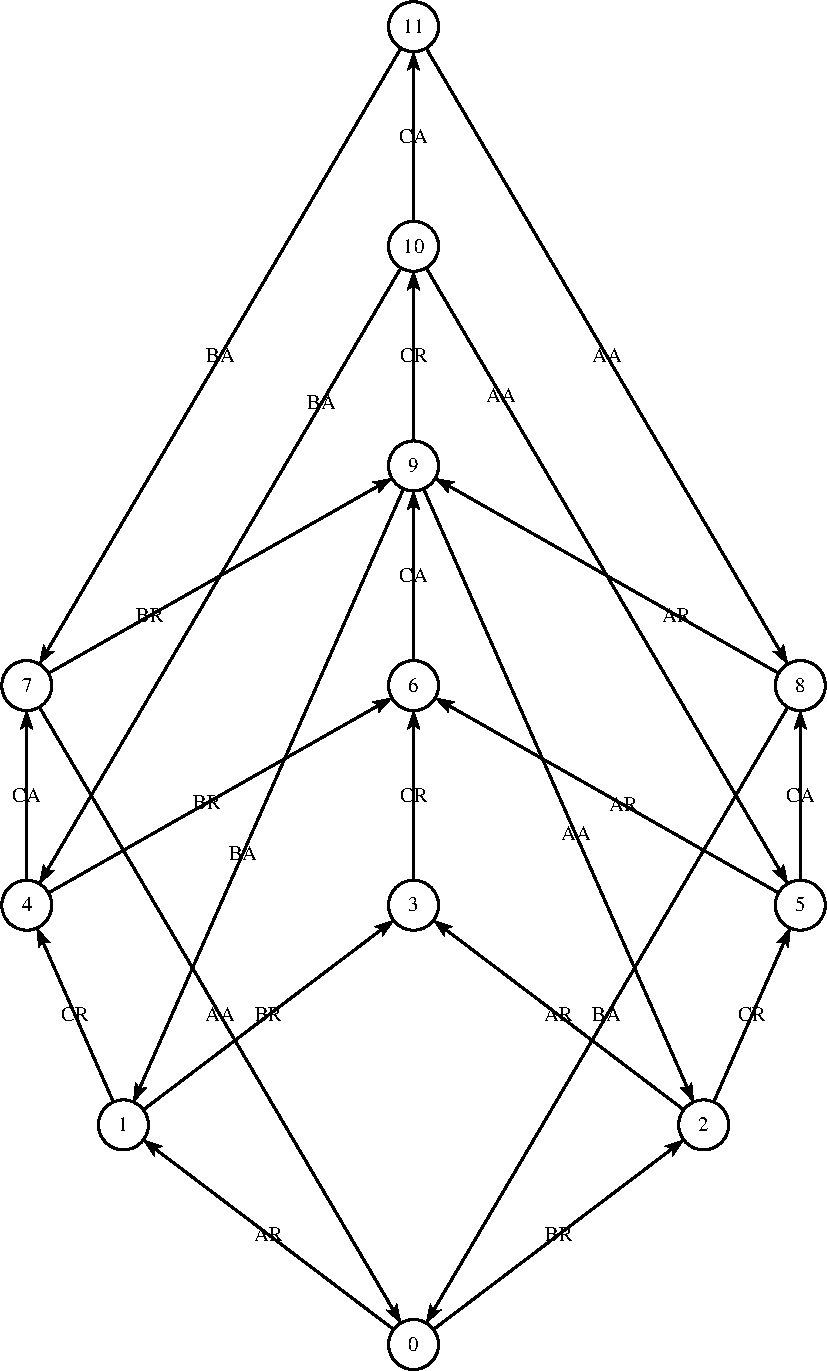
\includegraphics[angle=-90,scale=0.8]{mixer2}
	\captionof{figure}{Etykietowany graf przejść (LTS) po redukcji (\textit{safety equivalence reduction} $\rightarrow$ \textit{trace equivalence reduction}) -- graf identyczny jak graf zdefiniowany w~opisie XDI}
	\end{minipage}
\end{figure}
%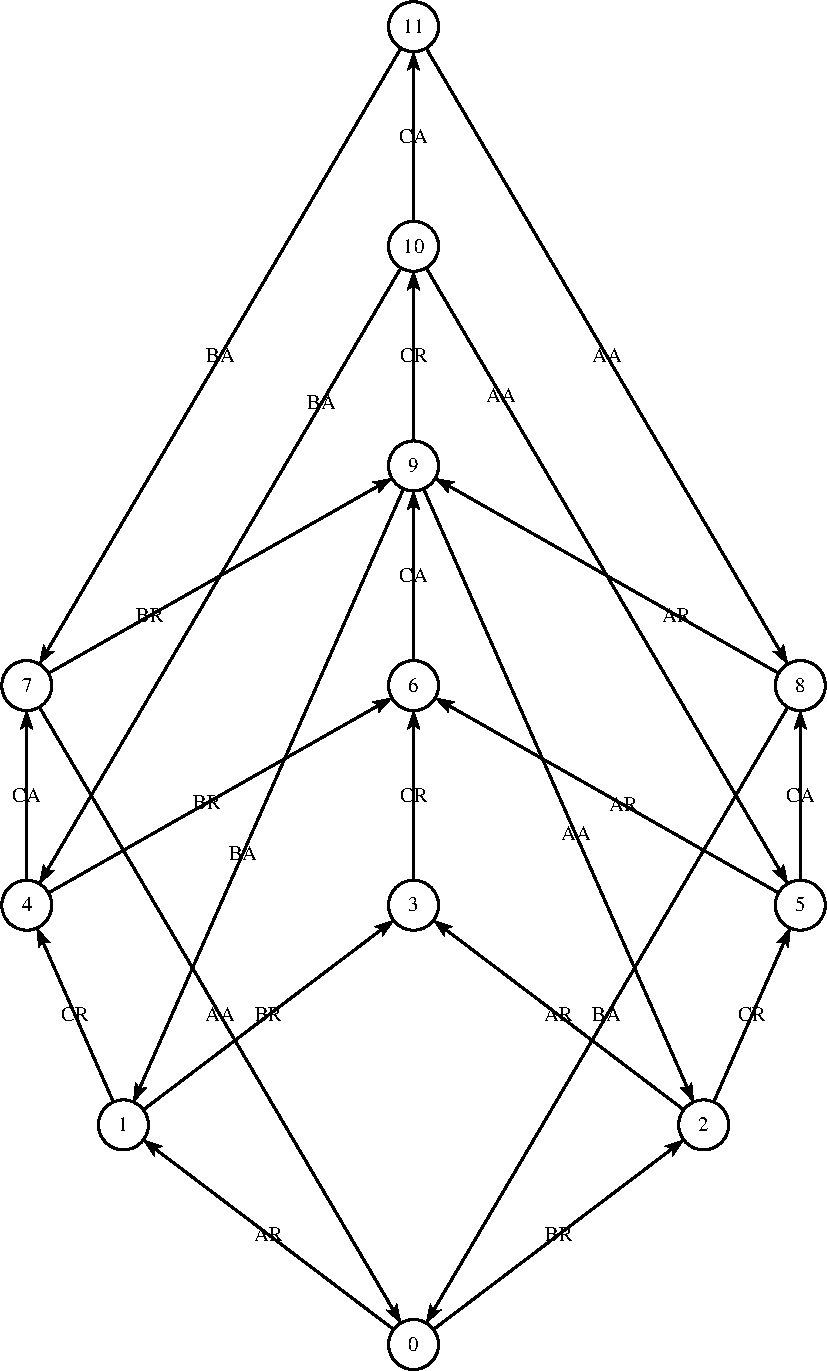
\includepdf[pages={-},angle=-90]{mixer2}

\end{document}
